\documentclass[a4paper]{article}
\usepackage{graphicx} % Required for inserting images
\usepackage{multicol}
\usepackage{enumitem}%предостовляет много вариков списка
\usepackage[english, russian]{babel}
\usepackage{hyperref}
\usepackage[%
left=0.50in,%
right=0.50in,%
top=0.8in,%
bottom=1.0in,%
left=0.50in,%
paperheight=11in,%
paperwidth=8.5in,%
]{geometry}%
\makeatletter
\newcommand*{\rom}[1]{\expandafter\@slowromancap\romannumeral #1@}
\makeatother
\setcounter{page}{300}%добовляет нумерацию страниц
\renewcommand*\labelenumi{[\theenumi]}

\begin{document}
\begin{multicols}{2}

\begin{minipage}{.4\textwidth}
\includegraphics[width=\linewidth]{Fotki Latex/organs.jpeg}
\scriptsize
\caption{Figure 10. Examples of correctly predicted images
with\par their prediction heatmaps for "Overall percent of\par abnormal volume" parameter:\par
a) patient ID 13676, actual value 14 \par%, predicted value 14 %;
b) patient ID 2641, actual value 30\par %, predicted value 28 %;
c) patient ID 19415, actual value 34 }\\ %, predicted value 33 %. 
\end{minipage}

\begin{minipage}{.4\textwidth}
    \includegraphics[width=\linewidth]{Fotki Latex/organs2.jpeg}
    \scriptsize
\caption{Figure 11. Examples of incorrectly predicted\par "Overall percent of
abnormal volume"\par with corresponding prediction heatmaps.}\\%

\end{minipage}
\vspace{3 mm}
\scriptsize

\columnbreak%переносит на другой столбец
\normalsize

but "Overall percent of abnormal volume" parameter is
set to zero.

\begin{minipage}{.3\textwidth}
\includegraphics[width=\linewidth]{Fotki Latex/organ.jpeg}
\end{minipage}
\vspace{3 mm}
\scriptsize 

Figure 12. The patient’s right lung has been damaged, but "Overall\par
percent of abnormal volume" parameter is set to zero.\\
\par
\normalsize
A study of patient ID 426 in the CASE BROWSER [2]
found that the other parameter "Pleural Effusion. %
of hemithorax involved" is equal to 50 %. Also, four
sextants were annotated and have some lesions: Upper,
Middle, Lower Right and Lower Left Sextants. The right
lung is particularly badly damaged.\par
At least 44 such images with markup inconsistencies
were found. It is necessary to exclude them from the
training samples.\par
\textit{Simple consistency checks}
s between different CXR annotation markup parameters should be developed for
future research. It is necessary to pay attention not only
to the images, but also to the various textual descriptions
provided.\par
As a result, it was concluded that the high MAE value
is due to the following reasons:
\begin{itemize}[noitemsep]%позволяет делать точки
\item background noise (outside the lungs) that requires
mask cropping to remove it;
\item the presence of artifacts in the lungs that requires
more data to train the neural network to correctly
distinguish these artifacts;
\item some errors in CXR image annotations that should
be excluded from the dataset.
\end{itemize}

\centerline{\rom{7}. Discussion of the application of semantic}
technologies in the context of the tasks considered in
\centerline{this paper}\par
In 1982, Japanese scientists developed a program for
the fifth generation of electronic computing machines.
Despite the fact that more than 42 years have passed,
the fifth generation computers have not been fully realized. The main difficulty in creating fifth-generation
computers or future computers is to create a machine
with artificial intelligence (AI) that will be able to draw
logical conclusions from the facts presented.\par
To interact with a fifth-generation computer, a person
(user) will not need to develop software for the machine

\end{multicols}
\begingroup
\begin{multicols}{2}
to solve the task at hand. In addition, fifth generation
computers will solve the problem of data formalization
in the interaction between computer and computer and
human and computer. Commands for the machine can be
formulated in ordinary spoken language without knowledge of formal programming languages as well as input
and output data formats.\par
Thus, fifth-generation computers are intelligent semantic systems with extremely high interoperability. Interoperability is the ability of a product or system, whose
interfaces are completely open, to interact and function
with other products or systems without any access or
implementation restrictions.\par
Although fifth generation computers have not yet been
realized, active work is being done to remove the barriers
between humans and computers, and between computers
and computers.\par
One of the directions for the development of interoperable intelligent computer systems is automatic
data transformation between different modalities: image
to text, text to image, speech to text, text to speech,
image to speech, speech to image, image to music, 3D
reconstruction of an object from a set of images, CT
scan to X-ray image, satellite image to geographical map,
geographical map to satellite image and other modality
transformations [19], [20].\par
This research project is developing an intelligent semantic system that converts a textual description into an
image, namely the textual markup of a radiologist into a
heatmap of lesion foci in the corresponding CXR medical
image.\par
A neural network trained to solve such a problem will
be a decision support system for population screening.
The trained neural network model will produce a textual
description of lung lesions based on the patient’s chest
radiograph, as well as a heatmap corresponding to these
lesions in the form of a graphical representation Fig.\ref{fig:Fotki1}13.

\begin{cupfigure}{}
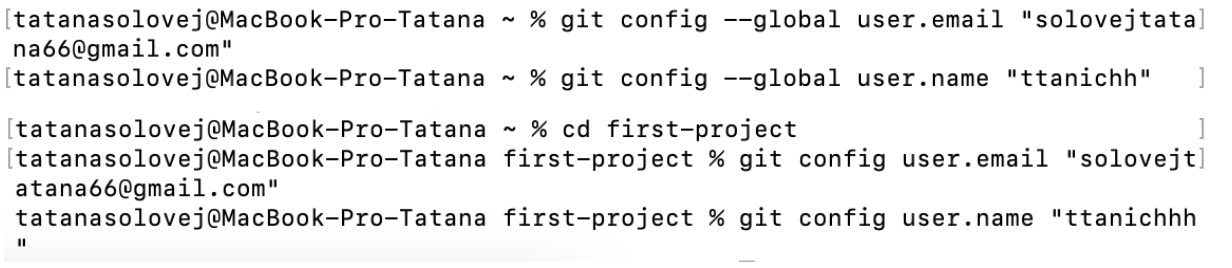
\includegraphics[width=0.9\linewidth, height=3cm]{Fotki Latex/13.jpeg}
\scriptsize 
    \caption{Figure 13. Operation schematic of the CXR-based decision support system under development.}
    \label{fig:Fotki1}
\end{cupfigure}
    
\normalsize\\
The problem of generating a heatmap from a textual
description and the subsequent problem of generating a
heatmap and corresponding textual description from an
input CXR image is one of the challenges of semantic
image segmentation.\par
Semantic image segmentation is the task of dividing
parts of an image into subgroups of pixels belonging to
corresponding objects, with subsequent classification of
these objects. Unlike classification and object detection
\columnbreak
tasks, the task of semantic segmentation is more complex
both in terms of solution methods and computational
resources [21].\par
Analyzing the literature to identify different semantic
methods for medical image processing revealed the following approaches:
\begin{itemize}[noitemsep]
    \item probabilistic latent semantic analysis (PLSA), which, in conjunction with neural network, is able to mining the hidden semantics of an image [22];
    \item implementation of Semantic Similarity Graph Embedding (SSGE) framework, which explicitly explores the semantic similarities among images [23];
    \item investigation and development of the concept of a personal intellectual assistant (secretary, referent) [24].
\end{itemize}\par
  Unfortunately, this paper does not apply the found
semantic methods to medical image processing. However,
the application of such semantic techniques in the context
of the tasks considered in this paper is very relevant in
future investigations.\par
As correctly noted in [25], "Currently, decision support systems in radiation mammology focus on the detection and classification of neoplasms, despite the
fact that{\it the real work of a radiologist does not imply
a diagnosing}. Computer vision systems use {\it a black box
model} and do not explain the results of work, which is
unacceptable in medicine".\par
This study also focuses on a deeper evaluation of
the behavior of such a "black box" (neural network
model) by studying the activation heatmaps on different
convolutional layers of the neural network, which are
obtained using the Gradient-weighted Class Activation
Mapping (Grad-CAM) method [18]. The investigation
of heatmaps on different convolutional layers provides
a better understanding of the decision-making logic of
the neural network based on the input data.\par
Fig. 5 shows the result of the semantic analysis of
lesion names. As shown in Fig. 5, there are four classes
of lesions: "Cavity", "Density", "Nodule" and "Collapse".
Meanwhile, the two classes "Density" and "Nodule" have
meaning overlap in the three lesion names. In the future,
semantic analysis methods will be applied to better
understand the disease asymmetry of different lung lobes
(see Tab. II).\par
After the decision support system for population
screening is completed, it is planned to be implemented into the already existing software "AI-based
software for computer-assisted diagnosis of lung diseases using chest X-Ray and CT images" (LungExpert,
https://lungs.org.by).\\

\centerline{\rom {8}. Conclusions}
\vspace{3 mm}
In this article, text annotations to CXR images were
analyzed. At this stage of the project, the main efforts of
the authors were focused on the formation of databases

for further research. A catalogue tree with new datasets
is described and constantly developing.\par
Two main tasks based on radiologists’ textual annotations were planned and the corresponding pipeline for the neural networks training was described: pulmonary disease study using sextants and the pulmonary disease
study using overall characteristics.\par
The task of predicting the parameter "Overall percent
of abnormal volume" showed that it is necessary to
develop additional simple consistency checks between
different CXR textual annotations. Also using lung masks
is a good idea to improve the quality of neural networks.
Further research is planned to create neural network
attention heatmaps based on the textual descriptions of
radiologists.\\
\par
\centerline{Acknowledgment}
\vspace{2 mm}
This work was carried out with the financial support of
the ISTC-PR150 "Belarus TB Database and TB Portal"
project.\\
\par

\centerline{Reference}

\begin{enumerate}
    \item TB Portals. Available at: https://tbportals.niaid.nih.gov (accessed
2024, March)
    \item CASE BROWSER. Available at:https://data.tbportals.\\niaid.nih.gov (accessed 2024, March)
    \item TB DEPOT. Available at: https://depot.tbportals.niaid.\\nih.gov/#/
cohort-creation?tab=4 (accessed 2024, March)
    \item Tuberculosis (pulmonary manifestations). Available at:
https://radiopaedia.org/articles/tuberculosis-pulmonarymanifestations-1 (accessed 2024, March)
    \item Statistical Atlas of Lung Lesions. Available at:
https://image.org.by/lesionAtlas (accessed 2024, March)
    \item V. Kovalev, V. Liauchuk, A. Gabrielian, A. Rosenthal, "Towards
Statistical Atlas of Lung Lesions," International Journal of
Computer Assisted Radiology and Surgery, 21-25 June, Munich, Germany, 2020, Vol. 15, Suppl. 1, pp. s31–s32. [Online].
Available: https://www.researchgate.net/publication/344217581\_
\item D.M. Hansell, A.A. Bankier, H. MacMahon, T.C. McLoud,
Towards\_Statistical\_Atlas\_o\_Lung\_Lesions
    \item Lung cavity. Available at: https://en.wikipedia.org/wiki\\/Lung\_
cavity (accessed 2024, March)
    \item D.M. Hansell, A.A. Bankier, H. MacMahon, T.C. McLoud,
N.L. Müller, J. Remy, et al., "Fleischner Society:
Glossary of terms for thoracic imaging," Radiology,
2008, Vol. 246, No. 3, pp. 697–722. [Online]. Available:
https://doi.org/10.1148/radiol.2462070712
    \item D.M. Hansell, A.A. Bankier, H. MacMahon, T.C. McLoud, K. Loverdos, A. Fotiadis, C. Kontogianni, M. Iliopoulou,
M. Gaga, "Lung nodules: A comprehensive review on current
approach and management," Annals of Thoracic Medicine, 2019,
Vol. 14, Issue 4, pp. 226–238. [Online]. Available: https://www.
ncbi.nlm.nih.gov/pmc/articles/PMC6784443
    \item D.M. Hansell, A.A. Bankier, H. MacMahon, T.C. McLoud, G. Metry, G. Wegenius, B. Wikström, V. Källskog, P. Hansell,
P.G. Lindgren, H. Hedenström, B.G. Danielson, "Lung density
for assessment of hydration status in hemodialysis patients using the computed tomographic densitometry technique," Kidney
international, 1997, Vol. 52, Issue 6, pp. 1635–1644. [Online].
Available: https://doi.org/10.1038/ki.1997.496
    \item D.M. Hansell, A.A. Bankier, H. MacMahon, T.C. McLoud, Pulmonary infiltrate. Available at: https://en.wikipedia.org/wiki/
Pulmonary\_infiltrate (accessed 2024, March)
    \item D.M. Hansell, A.A. Bankier, H. MacMahon, T.C. McLoud, Collapsed Lung (Pneumothorax). Available at: https://www.
pennmedicine.org/for-patients-and-visitors/patient-information/
conditions-treated-a-to-z/collapsed-lung-pneumothorax
(accessed 2024, March).
    \item ’Timika score’ on x-rays may help identify complex TB
cases. Available at: https://www.auntminnie.com/imag\-inginformatics/artificial-intelligence/article/15635618/\\timika-scoreon-xrays-may-help-identify-complex-tb-cases (accessed 2024,
March)
    \item A. Chakraborthy, A.J. Shivananjaiah, S. Ramaswamy,
N. Chikkavenkatappa, "Chest X ray score (Timika score):
an useful adjunct to predict treatment outcome in tuberculosis,"
Advances in Respiratory Medicine, 2018, Vol. 86, No. 5, pp. 205–
210. [Online]. Available: https://doi.org/10.5603/ARM.2018.0032
    \item LungExpert. Available at: https://lungs.org.by (accessed 2024,
March).
    \item TB DEPOT Data Dictionary. Available at: https://depot.tbportals.
niaid.nih.gov/#/data-dictionary (accessed 2024, March)
    \item ImageNet. Available at: https://www.image-net.org (accessed
2024, March)
    \item R.R. Selvaraju, M. Cogswell, A. Das, R. Vedantam., D. Parikh,
D. Batra, "Grad-CAM: Visual Explanations from Deep Networks
via Gradient-Based Localization," International Journal of Computer Vision, 2020, Vol. 128, No. 2, pp. 336–359. [Online].
Available: https://doi.org/10.1007/s11263-019-01228-7
    \item Top 7 text-to-image generative AI models. Available at:
https://byby.dev/ai-text-to-image-models (accessed 2024, Apr)
    \item Rohit Kundu. Image Processing: Techniques, Types, \& Applications [2023]. Available at: https://www.v7labs.com/blog/imageprocessing-guide (accessed 2024, Apr).
    \item M. Arsalan, M. Owais, T. Mahmood, J. Choi, K.R. Park, "Artificial Intelligence-Based Diagnosis of Cardiac and Related Diseases," Journal of Clinical Medicine, 2020, 9(3):871, pp 1–27.
[Online]. Available: https://doi.org/10.3390/jcm9030871
    \item M.R. Zare, M. Mehtarizadeh, "An Ensemble of Deep Semantic
Representation for Medical X-ray Image Classification," 2021
55th Annual Conference on Information Sciences and Systems
(CISS), Baltimore, MD, USA, 2021, pp. 1–6. [Online]. Available:
https://www.doi.org/10.1109/CISS50987.2021.9400268
    \item B. Chen, Z. Zhang, Y. Li, G. Lu, D. Zhang, "Multi-Label Chest
X-Ray Image Classification via Semantic Similarity Graph Embedding," in IEEE Transactions on Circuits and Systems for Video
Technology, April 2022, vol. 32, no. 4, pp. 2455–2468. [Online].
Available: https://www.doi.org/10.1109/TCSVT.2021.3079900
    \item V. Rostovtsev, "Intelligent health monitoring systems,"
Otkrytye semanticheskie tekhnologii proektirovaniya
intellektual’nykh system [Open semantic technologies for
intelligent systems], 2023, pp. 237–240. [Online]. Available:
https://libeldoc.bsuir.by/\\handle/123456789/51289
    \item A. Kayeshko, A. Efimova, "Decision support system for breast
cancer screening," Otkrytye semanticheskie tekhnologii proektirovaniya intellektual’nykh system [Open semantic technologies
for intelligent systems], 2021, pp. 229–232. [Online]. Available:
https://libeldoc.bsuir.by/handle/123456789/45424
\end{enumerate}
    
 \begin{center}
 \textbf{
\centerline { ОБРАБОТКА РЕНТГЕНОВСКИХ}\
 ИЗОБРАЖЕНИЙ ГРУДНОЙ КЛЕТКИ НА ОСНОВЕ ТЕКСТОВЫХ АННОТАЦИЙ
\centerline{ РАДИОЛОГОВ}}
\end{center}
\begin{te}
 \centerline{Косарева А. А., Павленко Д. А.,Снежко Э. В.}
 \end{te}
\vspace{1 mm}

\begin{textit}
    \\Проанализировано более 11 000 рентгеновских снимков
грудной клетки и соответствующих им текстовых аннотаций, а также проведены первые пилотные исследования
по обработке изображений с учетом текстовых аннотаций
специалистов-рентгенологов. Разработан конвейер обработки изображений для базы данных и нейронной сети. Проведено прогнозирование параметра «Общий процент аномального объема», для которого средняя абсолютная ошибка
составила 11,073 при использовании нейросетевой модели
InceptionResNet50V2.
\end{textit}
\begin{flushright}
     Received 12.03.2024
 \end{flushright}
 \end{multicols}
  \end{document}
 
 
